%%%%%%%%%%%%%%%%%%%%%%%%%%%%%%%%%%%%%%%%%%%%%%%%%%%%%%%%%%%%%%%%%%%%%%%%%%
\subsection{Hybrid scheme} %%%%%%%%%%%%%%%%%%%%%%%%%%%%%%%%%%%%%%%%%%%%%%%
%%%%%%%%%%%%%%%%%%%%%%%%%%%%%%%%%%%%%%%%%%%%%%%%%%%%%%%%%%%%%%%%%%%%%%%%%%

The hybridized SBP-SAT formulation discretizes this problem into the form 
\begin{equation}
    \left[\begin{array}{cc}
        \textbf{M}             & \textbf{F} \\
        \textbf{F}^{\intercal} & \textbf{D}
    \end{array}\right] 
    \left(\begin{array}{c}
        \textbf{u} \\
        \symbf{\lambda}
    \end{array}\right) = 
    \left(\begin{array}{l}
        \bar{\textbf{g}} \\
        \gbd
    \end{array}\right),
    \label{eqn:hybrid_system}
\end{equation}

\noindent
and following from {\color{red} [cite]} we use the Schur complement, $
(\textbf{D} - \textbf{F}^{\intercal} \textbf{M}^{-1} \textbf{F}) 
\symbf{\lambda} = \gbd - \textbf{F}^{\intercal} \textbf{M}^{-1} 
\bar{\textbf{g}}$, to solve this system in two parts: the global problem,

\begin{subequations}
\begin{equation}
\symbf{\lambda}_{\textbf{A}} \coloneqq \gbd - \textbf{F}^{\intercal} \text{solve}(\textbf{M}, \bar{\textbf{g}})
\label{eqn:global_system_a}
\end{equation}
\begin{equation}
\symbf{\lambda}_{\textbf{b}} \coloneqq \textbf{D} - \textbf{F}^{\intercal} \text{solve}(\textbf{M}, \textbf{F})
\label{eqn:global_system_b}
\end{equation}
\begin{equation}
\symbf{\lambda} \coloneqq \text{solve}(\symbf{\lambda}_{\textbf{A}}, \symbf{\lambda}_{\textbf{b}}),
\label{eqn:global_system_c}
\end{equation}
\end{subequations}
\noindent
and the local problem,
\begin{equation} 
\textbf{u} \coloneqq \text{solve}(\textbf{M}, (\bar{\textbf{g}} - \textbf{F} \times \symbf{\lambda})).
\label{eqn:local_system}
\end{equation}

\noindent
In this scheme, multiple elements with continuous domains can be coupled 
with boundary coefficients, similar to fluxes found in finite element 
methods. The boundary coefficients are factored out to $\textbf{F}$ and 
$\textbf{F}^{\intercal}$, leaving $\textbf{M}$ with a block diagonal 
non-zero pattern. 

\begin{aside}
	In this work we consider a specialization of the problem where the 
	number of elements, $\ell^2$, is the square of the number of elements
	on either side of the \emph{global} domain, $\ell$. Additionally, 
	each the number of volume points in each element, $n^2$, is the 
	square of the number of volume points along any side $n$. Finally, 
	there are only 4 interfaces, 1 for each orthogonal face of an element.
\end{aside}

\begin{figure}
	\centering
	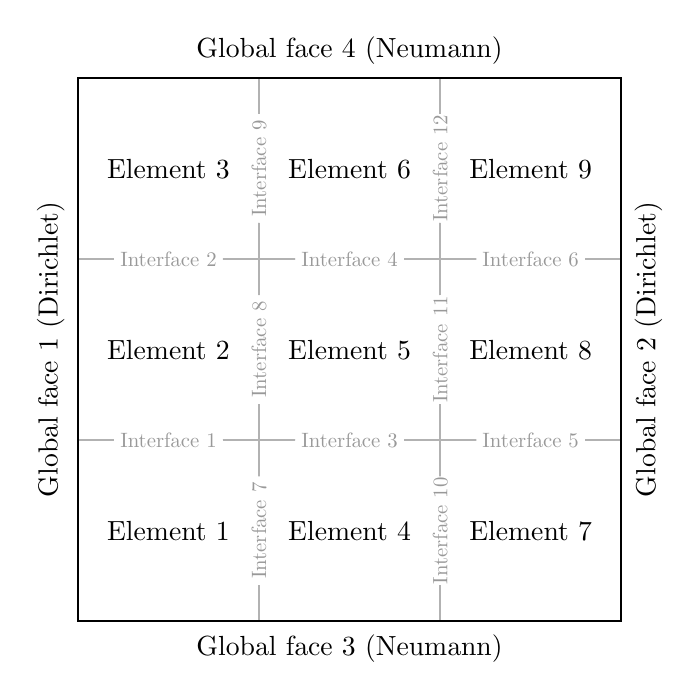
\begin{tikzpicture}[scale=2.3]
\draw[step=1cm,black!30,line width=0.3mm] (0, 0) grid (3, 3);
\draw[line width=0.3mm] (0, 0) rectangle (3, 3);

\fill[white] (0.5cm, 1cm) circle (0.3cm);
\node[color=black!40, scale=0.75] at (0.5cm, 1cm) {Interface 1};
\fill[white] (0.5cm, 2cm) circle (0.3cm);
\node[color=black!40, scale=0.75] at (0.5cm, 2cm) {Interface 2};
\fill[white] (1.5cm, 1cm) circle (0.3cm);
\node[color=black!40, scale=0.75] at (1.5cm, 1cm) {Interface 3};
\fill[white] (1.5cm, 2cm) circle (0.3cm);
\node[color=black!40, scale=0.75] at (1.5cm, 2cm) {Interface 4};
\fill[white] (2.5cm, 1cm) circle (0.3cm);
\node[color=black!40, scale=0.75] at (2.5cm, 1cm) {Interface 5};
\fill[white] (2.5cm, 2cm) circle (0.3cm);
\node[color=black!40, scale=0.75] at (2.5cm, 2cm) {Interface 6};

\fill[white](1cm, 0.5cm) circle (0.3cm);
\node[color=black!40, rotate=90, scale=0.75] at (1cm, 0.5cm) {Interface 7};
\fill[white] (1cm, 1.5cm) circle (0.3cm);
\node[color=black!40, rotate=90, scale=0.75] at (1cm, 1.5cm) {Interface 8};
\fill[white] (1cm, 2.5cm) circle (0.3cm);
\node[color=black!40, rotate=90, scale=0.75] at (1cm, 2.5cm) {Interface 9};
\fill[white] (2cm, 0.5cm) circle (0.3cm);
\node[color=black!40, rotate=90, scale=0.75] at (2cm, 0.5cm) {Interface 10};
\fill[white] (2cm, 1.5cm) circle (0.3cm);
\node[color=black!40, rotate=90, scale=0.75] at(2cm, 1.5cm) {Interface 11};
\fill[white] (2cm, 2.5cm) circle (0.3cm);
\node[color=black!40, rotate=90, scale=0.75] at (2cm, 2.5cm) {Interface 12};


\draw (0.5cm, 0.5cm) -- (0.5cm, 0.5cm) node[anchor=center] {Element 1};
\draw (0.5cm, 1.5cm) -- (0.5cm, 1.5cm) node[anchor=center] {Element 2};
\draw (0.5cm, 2.5cm) -- (0.5cm, 2.5cm) node[anchor=center] {Element 3};
\draw (1.5cm, 0.5cm) -- (1.5cm, 0.5cm) node[anchor=center] {Element 4};
\draw (1.5cm, 1.5cm) -- (1.5cm, 1.5cm) node[anchor=center] {Element 5};
\draw (1.5cm, 2.5cm) -- (1.5cm, 2.5cm) node[anchor=center] {Element 6};
\draw (2.5cm, 0.5cm) -- (2.5cm, 0.5cm) node[anchor=center] {Element 7};
\draw (2.5cm, 1.5cm) -- (2.5cm, 1.5cm) node[anchor=center] {Element 8};
\draw (2.5cm, 2.5cm) -- (2.5cm, 2.5cm) node[anchor=center] {Element 9};


\node[rotate=90] at (-0.15cm, 1.5cm) {Global face 1 (Dirichlet)};
\node[rotate=90] at (3.15cm, 1.5cm) {Global face 2 (Dirichlet)};
\node at (1.5cm, -0.15cm) {Global face 3 (Neumann)};
\node at (1.5cm, 3.15cm)  {Global face 4 (Neumann)};
\end{tikzpicture}
	\caption{An illustration the volume, and arrangement of interfaces 
		described by a 3-by-3 instance of the hybrid problem specified 
		in \eqref{eqn:hybrid_system}.}
	\label{fig:volume_diagram}
\end{figure}

\noindent
This permits us to \textbf{a)} compute much larger problems with less 
memory, especially if the problem is largely homogeneous, and \textbf{b)} 
reduce the computational complexity of solving the system by instead 
solving several smaller systems. In both cases this allows us express the 
equations (\ref{eqn:global_system_a}--\ref{eqn:global_system_c}, 
\ref{eqn:local_system}) as a concatenation of smaller problems. 

To form the smaller problems we decompose the sub-matrices 
$\textbf{M}$, $\textbf{F}$, $\textbf{F}^{\intercal}$, and $\textbf{D}$. 
For example, as $\textbf{M}$ is block-diagonal, we store each non-zero 
block of $\textbf{M}$ as distinct matrices. A similar structure exists 
for $\textbf{F}$ and $\textbf{F}^{\intercal}$. 

In a 3-by-3 example of the problem we reconstruct $\textbf{F}$ from the 
representational matrix, $\textbf{F}^{\text{ind}}$, and the set of unique
$\textbf{F}^{i}$ sub-matrices, substituting the appropriate sub-matrix in
place of the integer value, \emph{i.e.},
\begin{subequations}
\begin{equation}
	\textbf{F} = \textbf{F}^{\text{ind}}\left[\textbf{F}^{i}/i\right] \text{ where } i \neq 0,
\end{equation}
\begin{equation}
	{\footnotesize
    \begin{array}{c}
        {\color{gray} \hspace{-1em} \textit{Interface index}} \\
        {\color{gray}
        \begin{array}{C{0.25em}C{0.5em}C{0.5em}C{0.5em}C{0.5em}C{0.5em}C{0.5em}C{0.5em}C{0.5em}C{0.5em}C{0.5em}C{0.5em}C{0.5em}C{0.5em}}
        {}&{1}&{2}&{3}&{4}&{5}&{6}&{7}&{8}&{9}&{10}&{11}&{12}&{}\\
        \end{array}} \\
        \textbf{F}^{\text{ind}} = \left[\begin{array}{cccccccccccc}
         4 &{·}&{·}&{·}&{·}&{·}& 2 &{·}&{·}&{·}&{·}&{·}\\
         3 & 4 &{·}&{·}&{·}&{·}&{·}& 1 &{·}&{·}&{·}&{·}\\
        {·}& 3 &{·}&{·}&{·}&{·}&{·}&{·}& 2 &{·}&{·}&{·}\\
        {·}&{·}& 4 &{·}&{·}&{·}& 1 &{·}&{·}& 2 &{·}&{·}\\
        {·}&{·}& 3 & 4 &{·}&{·}&{·}& 1 &{·}&{·}& 2 &{·}\\
        {·}&{·}&{·}& 3 &{·}&{·}&{·}&{·}& 1 &{·}&{·}& 2 \\
        {·}&{·}&{·}&{·}& 4 &{·}&{·}&{·}&{·}& 1 &{·}&{·}\\
        {·}&{·}&{·}&{·}& 3 & 4 &{·}&{·}&{·}&{·}& 1 &{·}\\
        {·}&{·}&{·}&{·}&{·}& 3 &{·}&{·}&{·}&{·}&{·}& 1 \\
        
        \end{array}\right] {\color{gray}
        \begin{array}{C{1em}}
        1 \\ 2 \\ 3 \\ 4 \\ 5 \\ 6 \\ 7 \\ 8 \\ 9
        \end{array}{\rotatebox[origin=c]{90}{\textit{Block index}}}} \\
    \end{array}}
\end{equation}
\begin{equation}
	\left\{\textbf{F}^{1},\textbf{F}^{2},\textbf{F}^{3},\textbf{F}^{4}
	\right\}.
\end{equation}
\end{subequations}



e store $\textbf{F}$ as a vector of vectors to compute $\textbf{M}^{-1}\textbf{F}$. That is, for each directional $\textbf{F}^k$ boundary we store a list of $N$ vectors

\begin{equation}
    \textbf{F}^k = \left[\textbf{f}^k_1 \cdots \textbf{f}^k_N\right] \in \mathbb{R}^{N \times N^2}.
\end{equation} 

\noindent
In our implementation each vector $\textbf{f}^k_i$ is a PETSc vector. This method is in contrast to storing $\textbf{F}$ contiguously, and allows for the computation of $\textbf{M}^{-1}\textbf{F}$ from the local matrices of $\textbf{M}$, stored similarly as

\begin{equation}
    \textbf{M} = \left\{\textbf{M}_1 \cdots \textbf{M}_p\right\} \in \mathbb{R}^{N_{E}N^2 \times N_{E}N^2}, p \leq E.
\end{equation} 

\noindent 
Where $p$ denotes the number of unique local matrix operators in $\textbf{M}$. 

With this we compute the intermediate result $\textbf{M}^{-1}\textbf{F}$, performing a linear solve of every unique local matrix operator, and every vector of every directional boundary coefficient matrix 

\begin{equation}
    \text{solve}(\textbf{M}_{i}, \textbf{F}^{k}_j) \text{  for }
    \begin{array}{l}
        0 < i \leq p, \\
        0 < j \leq N, \\
        0 < k \leq D. \\ 
    \end{array}
\end{equation}

\noindent
The resultant has a similar non-zero pattern as $\textbf{F}$, following the same symbolic block structure. In our implementation we solve this system through direct solvers made available through PETSc. 

\begin{aside}
    In the homogeneous Poisson equation we have assembled in 
    eq {\color{red} ?? } 

    \begin{equation}
        p = \begin{cases}
            N_{EF} &  0 \leq N_{EF} < 3 \\ 
            3 &  3 \leq N_{EF} \\ 
        \end{cases}.
    \end{equation} 

    \noindent 
    When $p = 3$ we have one unique $\textbf{M}_i$ for the elements 
    along the top Neumann boundaries, the bottom Neumann boundaries, 
    and the interior elements. Since $p$ is constant when 
    $E \geq 3$, computational complexity decreases \emph{weakly} 
    as the number of elements in the system increases. Additionally, 
    if we fix $N^2E^2$ and increase $E$, we decrease the size of 
    each solve.
\end{aside}

\noindent
The resultant $\textbf{M}^{-1}\textbf{F}$ is stored as $p \times D \times N$ PETSc vectors of length $N^2$, i.e.,
\begin{subequations}
\begin{equation}
    \textbf{M}^{-1}\textbf{F} = [\alpha_{111} \cdots \alpha_{ijk} \cdots \alpha_{NDp}] \in \mathbb{R}^{pDN \times N^2},
\end{equation}
\begin{equation}
    \alpha_{ijk} = \text{solve}(\textbf{M}_i, \textbf{f}_{j}^{k}).
\end{equation}
 This is used in the matrix product $(\textbf{F}^{\intercal}) \times (\textbf{M}^{-1}\textbf{F})$, computing
\begin{equation}
    \Phi = N \sum_{i = 1}^{E} (\phi_i^2)
\end{equation}
vector dot products s.t.,
\begin{equation}
    \textbf{F}^{\text{ind}} = \left[\textbf{f}^{\text{ind}}_1 \cdots \textbf{f}^{\text{ind}}_{E}\right] \in \mathbb{Z}^{E \times I},
\end{equation}
\begin{equation}
    \phi = \left[ \text{nnz}(\textbf{f}^{\text{ind}}_1) \cdots \text{nnz}(\textbf{f}^{\text{ind}}_E) \right] \in \mathbb{Z}^{E}.
\end{equation}
Thus we have 
\begin{equation}
    (\textbf{F}^{\intercal}) \times (\textbf{M}^{-1}\textbf{F}) = 
    \left[\begin{array}{c}
        \beta_{1 1 1} \cdots \beta_{\phi_1 \phi_1 N} \in \mathbb{R}^{\phi_1^2N} \\ 
        \vdots \\
        \beta_{1 1 1} \cdots \beta_{\phi_E \phi_E N} \in \mathbb{R}^{\phi_E^2N} 
    \end{array}\right] 
\end{equation}
\begin{equation}
    \beta_{i j k l} = \alpha_{iyl} \textbf{f}^{u}_{l}, \text{ where } y = \text{nzval}(\textbf{f}^{\text{ind}}_{ij}), u = \text{nzval}(\textbf{f}^{\text{ind}}_{ik}),
\end{equation}
\end{subequations}
where $\text{nzval}(v_i)$ returns the $i\text{th}$ non-zero value in the vector $v$. Notably here the result is not square of all non-zeros in $\textbf{F}^\text{ind}$, but the sum of the squares of each row in $\textbf{F}^\text{ind}$, making the storage dependent upon $p$, the number unique elements and the sparsity of $\textbf{F}$. 

The index for any scalar value $\beta_{i j k l}$ in the matrix representation of $\textbf{F}^{\intercal}\textbf{M}^{-1}\textbf{F}$ is given as 
\begin{equation}
[(N - 1) i + \text{nzind}(\textbf{f}^{\text{ind}}_{ij}) + l, (N - 1) i + \text{nzind}(\textbf{f}^{\text{ind}}_{ik}) + l]
\end{equation}
\noindent
where $\text{nzind}(v_i)$ returns the index of the $i\text{th}$ non-zero of the vector $v$. Since 
%\begin{}




\begin{figure}
    \centering
    \begin{center}
\begin{tikzpicture}
\begin{axis}[
  /pgf/number format/1000 sep={\,},
  height=2in,
    xlabel={\small $\ell^2$ (total elements)},
  width =3in,
  axis x line*=bottom,
  axis y line*=left,
  xtick={9, 144, 484, 1024},
  %ymode=log,
  ylabel={\small $\text{FLOP} / \text{byte}$}
  legend style={
    font=\footnotesize,
    at={(0.975, 0.05)},
    anchor=south east},
  legend cell align={left}]
    \addplot[
        select coords between index={1}{2500},
        color=black,smooth,thick] 
        table[col sep=comma,header=false,
        x index=0,y index=1] {data/ai_fmft};
\end{axis}
\end{tikzpicture}
\end{center}

    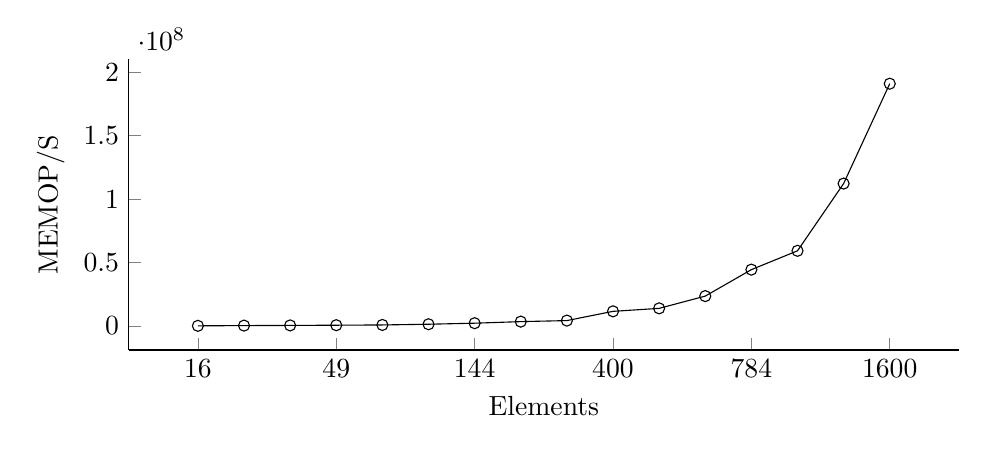
\begin{tikzpicture}
    \begin{axis}[
        height=15em,
        width=\linewidth,
        axis x line*=bottom,
        axis y line*=left,
        symbolic x coords = {16, 25, 36, 49, 64, 100, 144, 196, 225, 400, 441, 576, 784, 900, 1225, 1600},
        xtick = {16, 49, 144, 400, 784, 1600},
        ytick = {0, 5e7, 1e8, 1.5e8, 2e8},
        domain = 16:1600,
        range = 0:2e8,
        xlabel={Elements},
        ylabel={MEMOP/S}]
        \addplot[
            mark=o,
            color=black] coordinates {
            	(16, 102587.136429503)
            	(25, 290460.3459064985)
            	(36, 425601.69074644265)
            	(49, 593216.5799791333)
            	(64, 798987.4503421097)
            	(100, 1.3572377963761303e6)
            	(144, 2.1872863978127134e6)             	 
            	(196, 3.4170699854037026e6) 
            	(225, 4.234649395939718e6) 
            	(400, 1.1519383748304999e7) 
            	(441, 1.387318563789152e7) 
            	(576, 2.3530732528767895e7) 
            	(784, 4.440605746530777e7) 
            	(900, 5.9239537399118066e7) 
            	(1225, 1.1224531627926044e8)
            	(1600, 1.9097409512744978e8)		
            };
    \end{axis}
\end{tikzpicture}

    \caption{.}
    \label{fig:todo}
\end{figure}

